\begin{frame}[c]
    \frametitle{基于锥形空心布拉格波导的芯片级光谱测量}
    \begin{itemize}
        \item DeCorby, R. G.;  Ponnampalam, N.;  Epp, E.;  Allen, T.; McMullin, J. N., \textcolor{purple}{Chip-scale} spectrometry based on \textcolor{red}{tapered hollow Bragg waveguides}. Optics Express 2009, 17 (19), 16632-16645
        \item \textcolor{blue}{意义:}结合了法布里-珀罗谐振腔和光栅的优势。
    \end{itemize}
    仪器结构示意图:
    \begin{figure}[H] %H为当前位置,!htb为忽略美学标准,htbp为浮动图形
        \centering %图片居中
        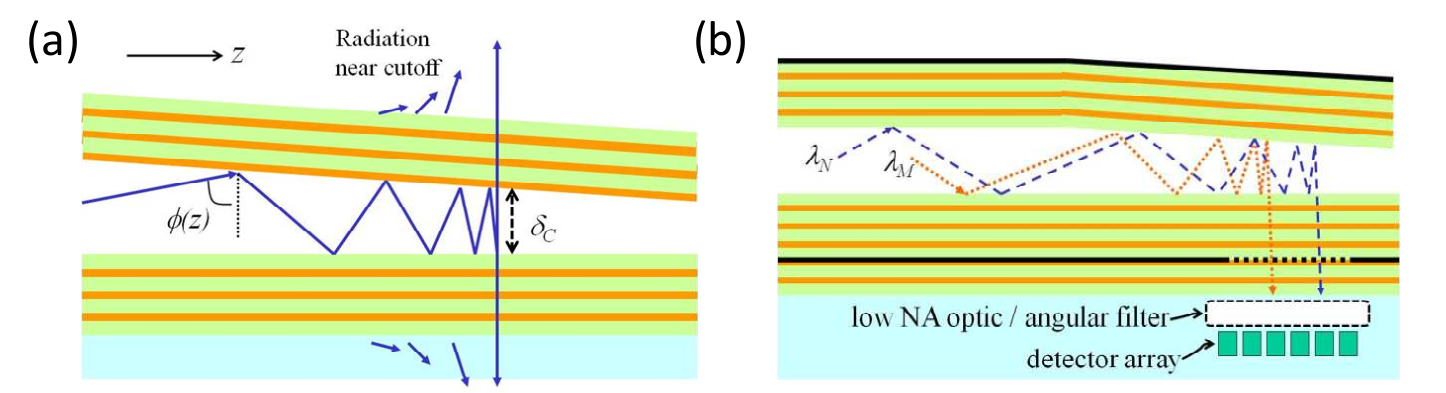
\includegraphics[width=1.\textwidth]{figures/Chip-scale spectrometry based on tapered hollow Bragg waveguides_1.png} %插入图片,[]中设置图片大小,{}中是图片文件名
    \end{figure}
    \begin{itemize}
        \item 原理:在某一截止位置处,特定的反射镜间距使得对应波长达到法布里珀罗谐振条件。
        \item 文章细节待读……
    \end{itemize}
\end{frame}